\begin{figure}[ht!]
\centering
\subfigure{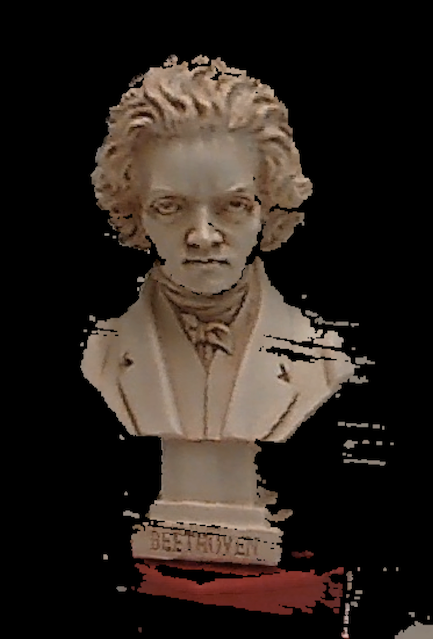
\includegraphics[width=.25\linewidth]{figures/results-1}}\quad
\subfigure{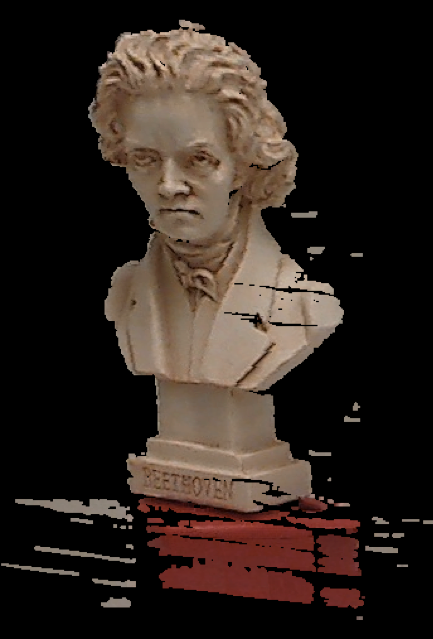
\includegraphics[width=.25\linewidth]{figures/results-2}}
\label{figure:results}
\caption{Results}
\end{figure}

The imaging system in addition to the source directory, expects a reference image without the laser stripe and two images of the individual background patterns used for calibration as input. The program saves the point cloud thus obtained in a destination directory which is used by the \ac{3DTK} components for processing and visualization as shown below. 

\begin{verbatim}
$ bin/projectionlaserscanner $SOURCE_DIR \
                             $REFERENCE_IMG \
                             $LEFT_CHECKERBOARD_PATTERN \
                             $RIGHT_CHECKERBOARD_PATTERN \
                             $DESTINATION_DIR \
$ bin/slam6D $DESTINATION_DIR
$ bin/show $DESTINATION_DIR
\end{verbatim}

The results thus obtained from the \texttt{show} program are shown in figure \ref{figure:results}.